\begin{figure*}[t]
\centering
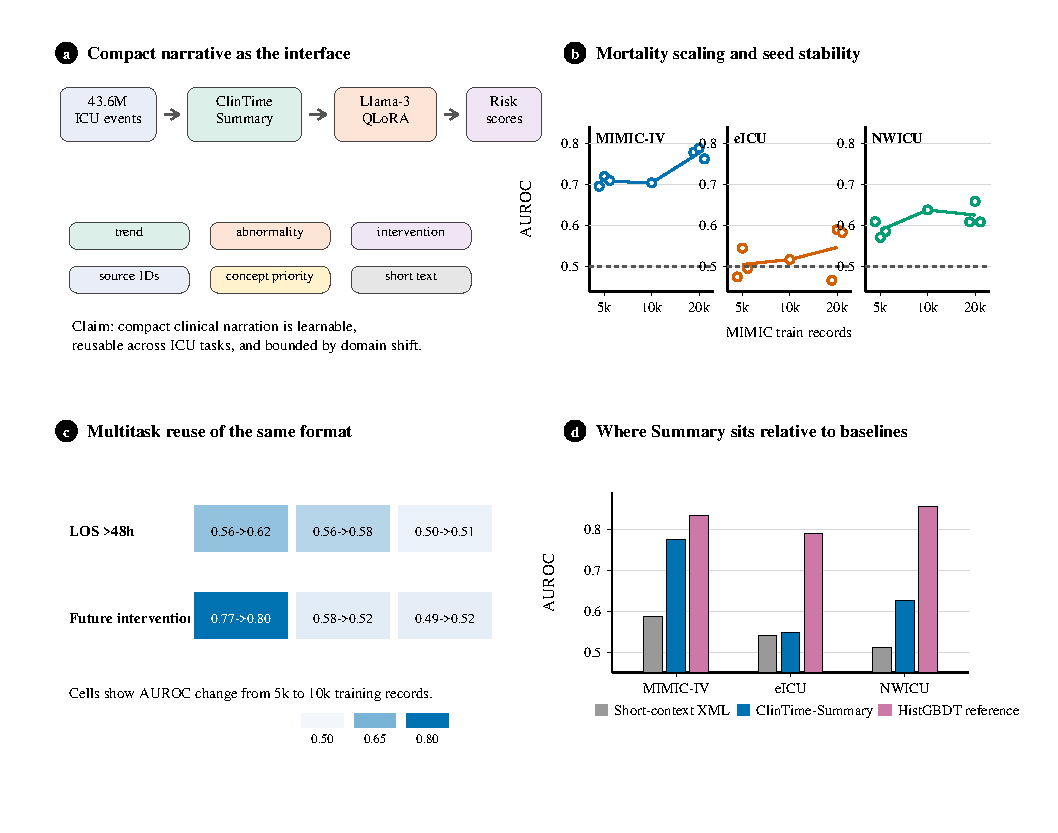
\includegraphics[width=0.98\textwidth]{figures/fig_summary_main_composite.pdf}
\caption{Main evidence for ClinTime-Summary. (a) The representation compresses source-linked ICU events into prioritized clinical narratives before Llama-3-8B QLoRA prediction, preserving trend, abnormality, intervention, and provenance cues. (b) Mortality AUROC improves with larger MIMIC-IV training sets and remains stable over the completed 20k seeds; points indicate individual seeds and lines indicate means. (c) The same narrative format transfers to auxiliary ICU endpoints, with cells showing AUROC changes from 5k to 10k records. (d) ClinTime-Summary substantially closes the short-context XML gap while remaining below the supervised HistGBDT data-validity reference, motivating a bounded claim rather than a clinical-superiority claim.}
\label{fig:summary_main}
\end{figure*}
